% ============================================================
% Cleveland & McGill (1984) perceptual hierarchy
% Vector PDF figure imported from the figures/ directory.
%
% Requires:
%   cleveland_preview.pdf
%
% (\graphicspath{{figures/}} is already defined in main.tex)
% ============================================================

\begin{figure}[!ht]
    \centering
    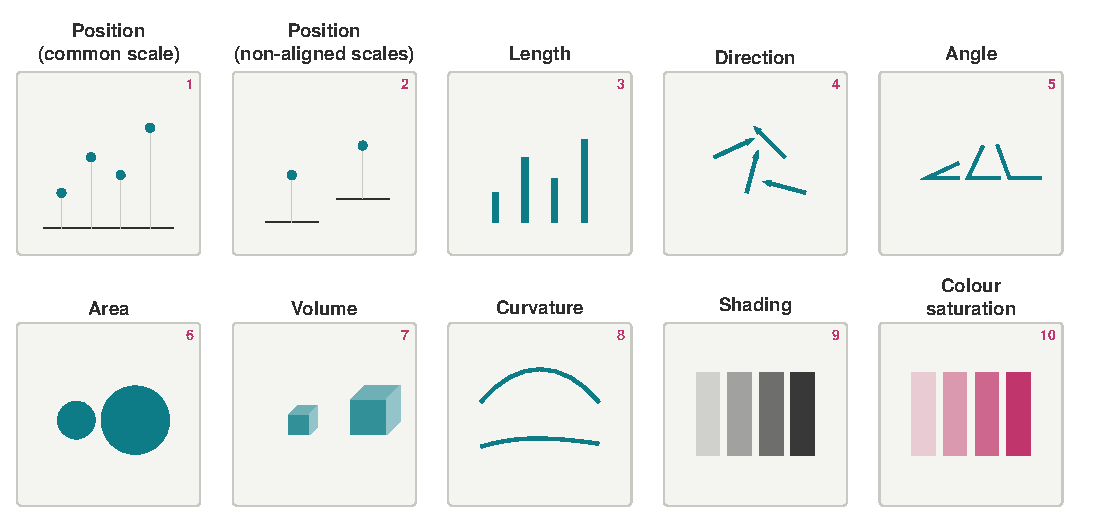
\includegraphics[width=\textwidth]{figures/literature/cleveland_preview.pdf}
    \caption[The Cleveland \& McGill hierarchy of perceptual tasks.]{\textbf{The hierarchy of elementary perceptual tasks, after \citet{clevelandmcgill1984}.}
    Encodings are ordered by decoding accuracy, from most accurate (1, position on
    a common scale) to least accurate (10, colour saturation). The ranking is
    empirical, not aesthetic: it reflects how accurately people extract a
    quantitative value from each visual channel. It underlies design-grammar
    principle~P0 (Table~\ref{tab:design-grammar}) --- assign the most important
    variable to the most accurately decoded channel --- and principle~P1, which
    places continuous magnitude on spatial position.}
    \label{fig:perceptual-hierarchy}
\end{figure}